%BAB_3 LAPORAN KP

\chapter{PERANCANGAN SISTEM}
Pada bab ini akan disajikan mekanisme perancangan alat, baik perangkat keras ataupun perangkat lunak untuk mewujudkan sebuah robot lengan. Tahapan perancangan dimulai dari perancangan diagram blok sistem, perancangan perangkat keras, perancangan perangat lunak, perancangan kinematika balik, dan integrasi keseluruhan program. 
\section{ Diagram Blok Sistem }
Secara garis besar, pada tahapan implementasi dari kinematika pada \textit{arm manipulator robot} SCARA ini menggunakan output atau penggerak berupa motor DC dengan \textit{feedback} posisi berupa potensiometer dan pada bagian  input yang berasal dari Processing IDE yang mengirimkan sebuah koordinat yang digunakan untuk menentukan pergerakan robot berdasarkan fungsi \textit{inverse kinematic}. Sistem kerja \textit{arm manipulator robot} SCARA ditunjukan pada  Gambar 3.1.
\begin{figure}[H]
	\centering
	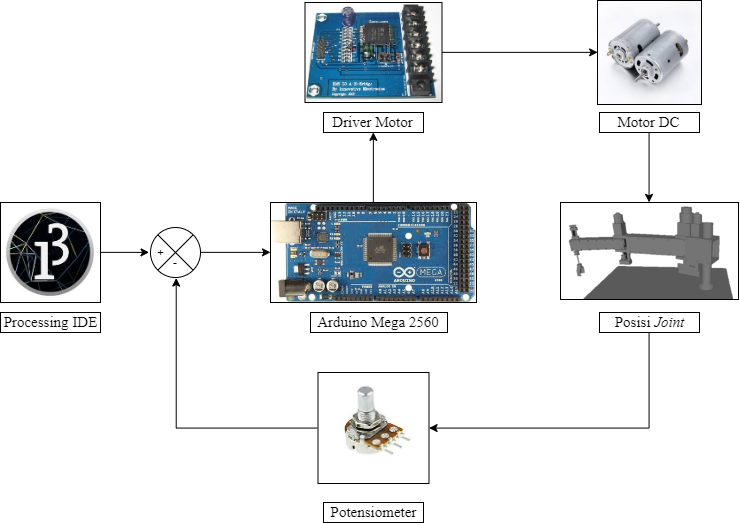
\includegraphics[width=12cm]{gambar/Rangkaian_Diagram.png}
	\caption{Diagram Blok Sistem}
\end{figure}
Pada blok diagram yang disajikan pada Gambar 3.1 sistem terdiri dari bagian – bagian yang meliputi bagian masukan, bagian kendali, bagian keluaran, dan bagian penampil. Pada bagian masukan menggunakan GUI yang dirancang pada Processing IDE yang digunakan sebagai \textit{forward kinematic} serta \textit{inverse kinematic} dimana robot akan bergerak menyesuaikan dengan posisi atau sudut yang diinputkan melauli Processing IDE. 
Pada bagian kontrol menggunakan Arduino Mega 2560 sebagai mikrokontroler yang mengendalikan seluruh operasi dari robot. \textit{Power supply} Arduino sebesar 5 volt DC didapatkan dari regulator tegangan yang menurunkan tegangan dari 12 volt DC ke 5 volt DC. 

Pada bagian keluaran, pin pulse with modulation (PWM) pada Arduino Mega 2560 dihubungkan dengan driver motor yang digunakan untuk mengontrol arah pergerakan dari motor DC serta kecepatan pergerakan dari motor DC. Pergerakan arah putaran motor DC bergantung pada \textit{feedback} posisi setiap sendi yang diberikan oleh potensiometer. Tiga buah pin digital ardunio dihubungkan rangkaian \textit{switch} yang menggunakan IC TIP31 yang berfungsi sebagai kontrol dari \textit{End-Effector} dari robot SCARA.

Pada bagian penampil merupakan bentuk dari rancangan GUI yang dirancang dalam Processing IDE melalui sebuah bentuk pemrograman. Dalam tampilan GUI nya, terdapat beberapa \textit{tools} yang dapat untuk mengatur pergerakan robot SCARA. Pada GUI juga dapat menampilkan nilai dari sudut, dan posisi pada kondisi langsung dari pergerakan robot SCARA.
\section{ Perancangan Perangkat Keras }
Perancangan perangkat keras pada \textit{arm manipulator robot} SCARA terdiri dari dua bagian yaitu bagian mekanik dan elektronis. Bagian  mekanik merupakan bagian \textit{hardware} yang meliputi desain, bahan dan bentuk dari arm manipulator robot SCARA dan bagian elektronis merupakan bagian \textit{hardware} yang meliputi sistem – sistem yang berkaitan dengan rangkaian pada I SCARA seperti rangkain pada desain \textit{board} serta komponen – komponen elektronis.
\subsection{ Sistem Mekanik }
Sistem mekanika dari robot lengan bergantung dari konfigurasi robot lengan. Konfigurasi robot lengan terbagi menjadi enam, yaitu konfigurasi \textit{Articulated}, konfigurasi SCARA, konfigurasi \textit{Spherical}, konfigurasi \textit{Cylindrical}, dan konfigurasi \textit{Cartesian}. Pada tugas ini, konfigurasi robot lengan yang digunakan adalah konfigurasi SCARA, dengan dua joint revolute dan satu \textit{end-effector}. Sistem mekanik dari lengan robot tiga DOF sangat berpengaruh dan mendominasi sistem karena bentuk dan pergerakan dari mekanik akan mempengaruhi elektronis, serta program. Sistem mekanik yang baik sangat mendukung dari pergerakan robot, oleh karena itu perancangan mekanik haruslah proporsional dari panjang setiap lengan, lebar serta tinggi robot. Pada Gambar 3.2 disajikan \textit{free body} dari robot SCARA dan Gambar 3.3 merupakan bentuk fisik dari robot SCARA yang digunakan pada penelitian kali ini.
\begin{figure}[H]
	\centering
	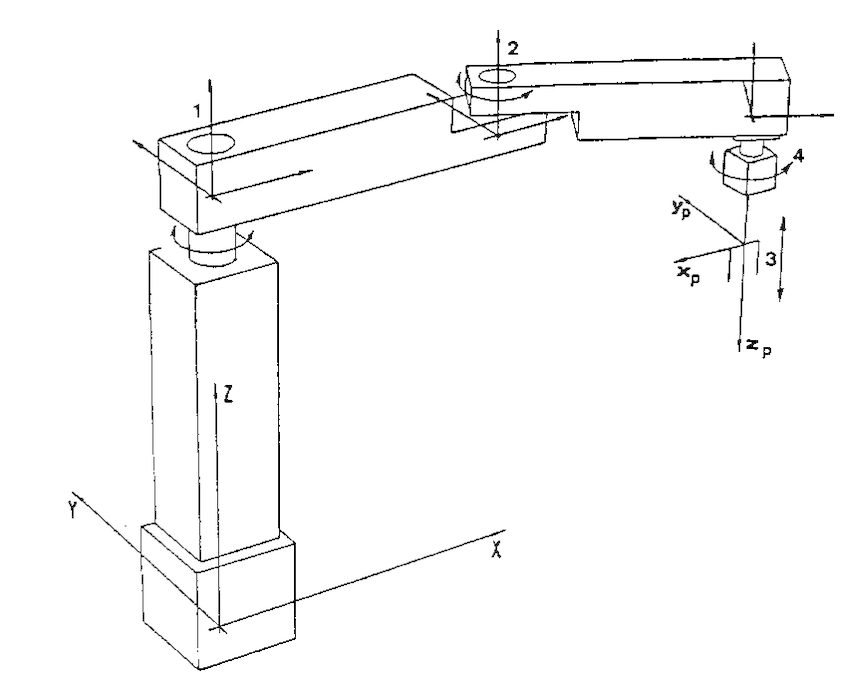
\includegraphics[width=7cm]{gambar/scaraa.png}
	\caption{\textit{Free Body} Robot SCARA}
\end{figure}
\begin{figure}[H]
	\centering
	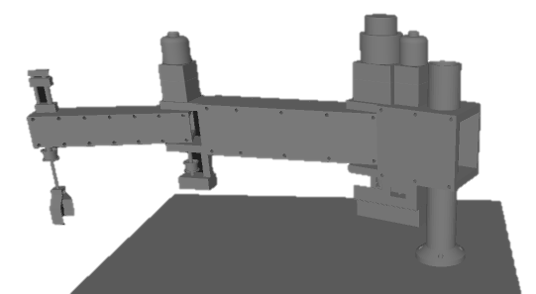
\includegraphics[width=7cm]{gambar/3dscara.png}
	\caption{Bentuk Fisik Robot SCARA}
\end{figure}
Robot SCARA merupakan robot yang meiliki tiga buah derajar kebebasan (DOF) yang terletak pada \textit{shoulder}, \textit{elbow}, dan pada \textit{end-effector}. Pada \textit{shoulder} dan \textit{elbow} menggunakan sebuah motor DC dan pada \textit{end-effector} menggunakan bantuan angin yang dikontrol penggunakan \textit{valve pneumatic.} Pergerakan pada masing-masing \textit{joint} memiliki jangkauan maksimum yang berbeda-beda. Jangkauan juga dipengaruhi oleh panjangnya lengan yang dimiliki oleh robot SCARA tersebut. Tabel 3.1 merupakan spesifikasi dari robot SCARA yang digunakan.


\begin{table}[H]
	\centering
	\caption{Spesifikasi Robot SCARA}
	
		\begin{tabular}{|l|l|}
			\hline
			Main arm length      & 360 mm		\\ \hline
			Fore arm length      & 290 mm  				\\ \hline
			Shoulder movement    & 180 °  		\\ \hline
			Elbow movement       & 200 °   		\\ \hline
			Wrist rotation       & 360 ° 		\\ \hline
			Up \& down movement  & 150 mm   				\\ \hline
			Maximum tip velocity & 3.0 kg  				\\ \hline
		\end{tabular} 
	\end{table}
Desain pada\textit{ arm manipulator robot} SCARA berbahan besi dengan tebal 2mm dengan tiga derajat kebebasan yang meliputi bagian \textit{shoulder}, \textit{elbow}, serta \textit{end-effector}. Pada desainnya robot SCARA terbagi menjadi dua bagian. Bagian utama adalah box panel yang berisi sistem elektronis utama dan pada bagian yang lain merupakan lengan dari robot SCARA sendiri. Terdapat juga tiga buah selang yang berfungsi untuk mentransformasikan angin untuk pergerakan dari \textit{end-effector} yang berasal dari sebuah kompresor.  Dalam komunikasinya dengan komputer personal, robot SCARA dihubungkan dengan konektor USB. Gambar 3.4 merupakan bentuk fisik dari box panel pada Robot SCARA.
\begin{figure}[H]
	\centering
	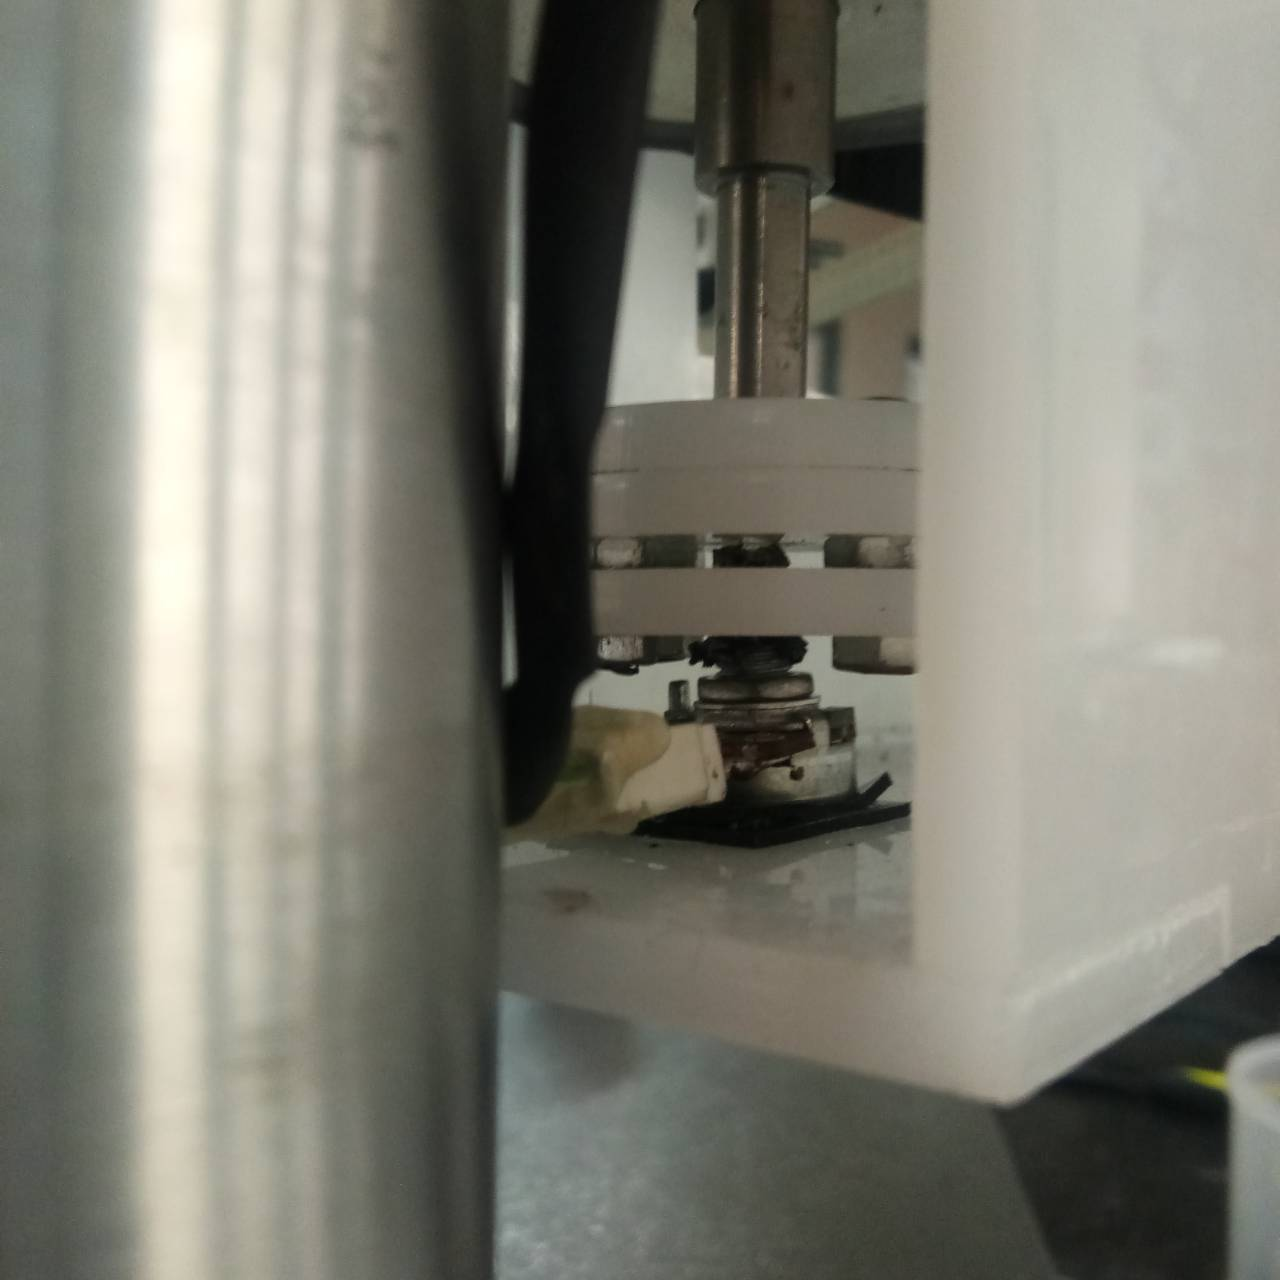
\includegraphics[width=7cm]{gambar/potsementara.jpg}
	\caption{Box Panel Robot SCARA}
\end{figure}

Pada \textit{arm manipulator robot} SCARA menggunakan penggerak berupa motor DC 12 Volt dengan diberikan \textit{gearbox} sehingga mampu mengangkat beban berat karena torsi pada motor bertambah besar. Motor DC dikontrol dari driver motor EMS 30A H-Bridge melalui mikrokontroler Arduino Mega 2560. Tabel 3.2 merupakan spesifikasi dari motor DC yang digunakan pada robot SCARA. 

	\begin{table}[H]
	\centering
	\caption{Spesifikasi Motor DC pada Robot SCARA}
	\resizebox{15cm}{!}{%
		\begin{tabular}{|l|l|}
			\hline
			Moments of inertia of the main arm ($J_{1}$)    							& $0.0980kgm^{2}$ 				\\ \hline
			Moments of inertia of the fore arm ($J_{2}$)    							& $0.0115 kgm^{2}$ 				\\ \hline
			Masses of the main arm	($m_{1}$)											& $1.90kg$   					\\ \hline
			Masses of the fore arm  ($m_{2}$)     										& $0.93kg$   					\\ \hline
			Motor and equivalent inertias ($J_{m}$)      								& $3.3*10^{-6}kgm^{2}$ 			\\ \hline
			Back emf constants for main arm and fore arm motor ($K_{e1}=K_{e2}$)  		& $0.047Nm/A$   				\\ \hline
			Armature resistance for main arm and fore arm motor($R_{a1}=R_{a2}$)		& $3.5\Omega$  					\\ \hline
			Armatures inductances for main and fore arm motor  ($L_{a1}=L_{a2}$) 		& $1.3mH$ 						\\ \hline
		\end{tabular}%
	}
\end{table}
%%
Pada bagian \textit{gearbox} pada masing-masing motor DC terdapat \textit{potensiometer} sebagai sensor posisi. \textit{Potensiometer} ditempatkan pada bawah motor DC yang terhubung langsung. Setiap pergerakan dari motor DC, \textit{potensiometer} akan secara otomatis juga ikut bergerak dan kemudian mengirimkan nilai data analog ke Arduino Mega. Nilai ini dalam Arduino Mega dilakukan sebuah perhitungan untuk menghasilkan sebuah posisi berupa besar sudut dari setiap motor DC saat dioperasikan. Gambar 3.5 merupakan bentuk fisik dari motor DC serta pemasangan \textit{potensiometer}.
\begin{figure}[H]
	\centering
	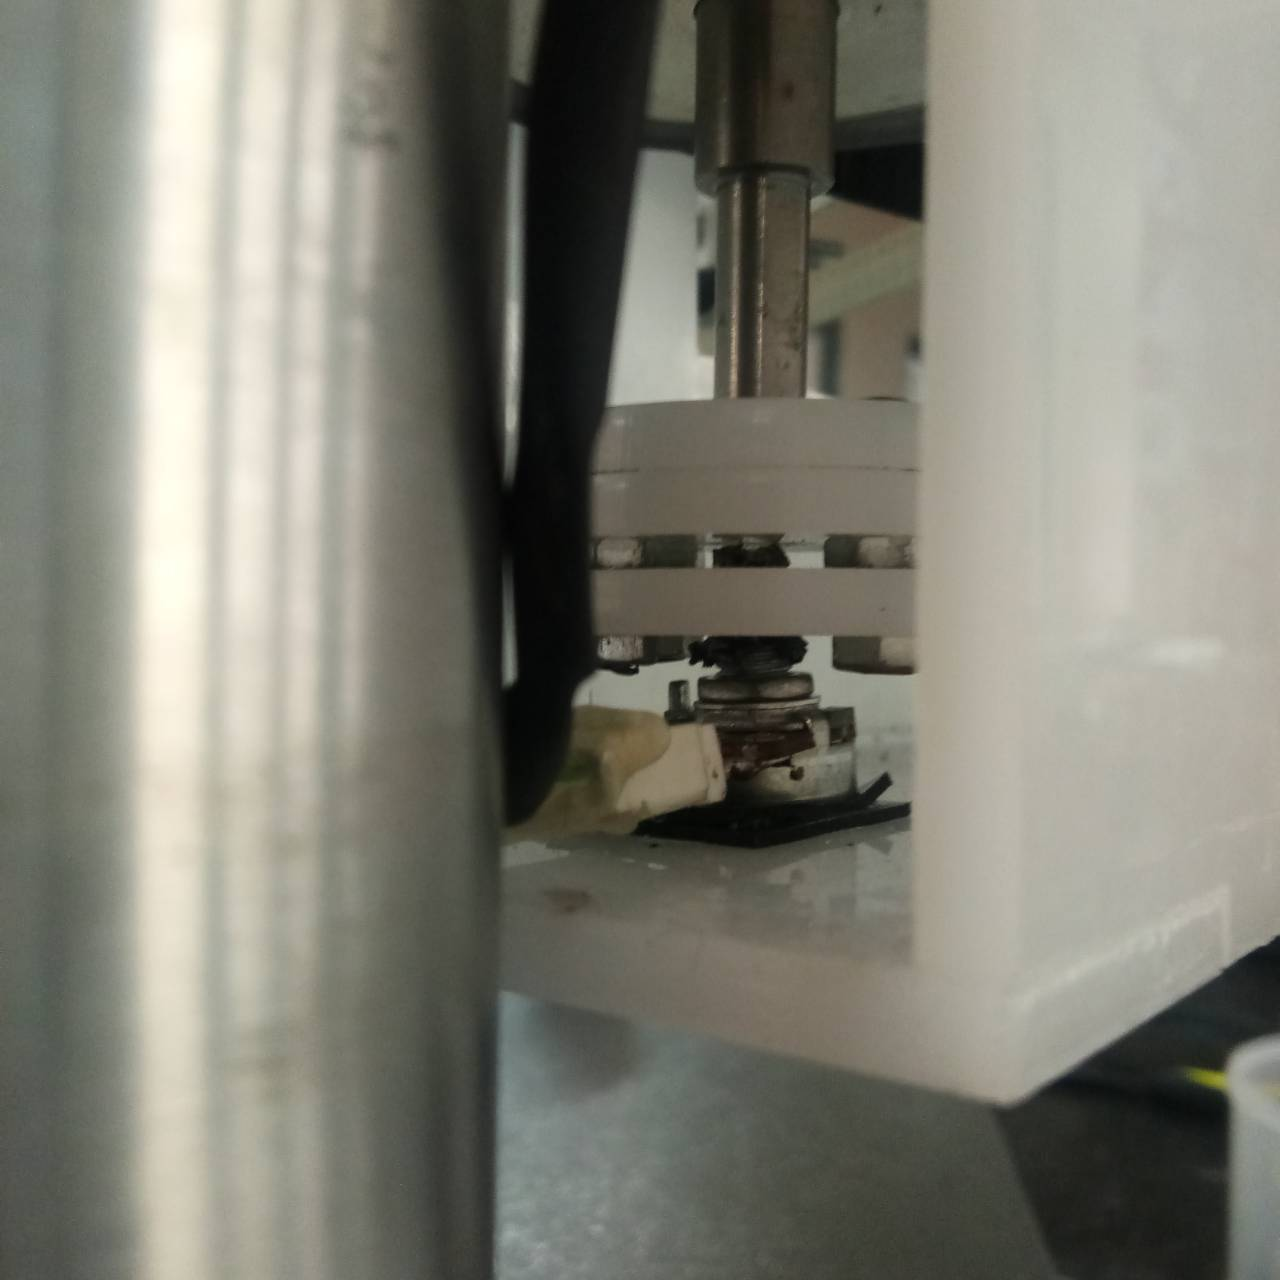
\includegraphics[width=7cm]{gambar/potsementara.jpg}
	\caption{Motor DC dengan Potensiometer}
\end{figure}

Pada bagian \textit{end-effetor} menggunakan pergerakan translasi. Pergerakan translasi merupakan pergerakan garis lurus dengan sebuah sumbu. Pada robot SCARA pergerakan ini ada pada bagian \textit{end-effector} yang bergerak secara vertikal atau naik turun. Dengan pergerakan ini, posisi \textit{end-effector} mengalami perubahan pada posisi tingginya. Pergerakan translasi juga terdapat pada bagian \textit{end-effector} yang menyebabkan sebuah\textit{ end-effector} dapat membuka dan menutup karena sebuah sistem mekanik yang telah ada. Selain dari pergerakan translasi, pergerakan pada end-effector juga terdapat rotasi. Pergerakan ini dilakukan oleh satu buah motor DC yang ditempatkan pada bagian base dengan dihubungkan melalui sebuauh belt. Pengoperasian pada motor DC ini juga dilakukan oleh driver motor EMS 30A H-Bridge. Gambar 3.6 merupakan bentuk fisik dari \textit{end-effector}. 
\begin{figure}[H]
	\centering
	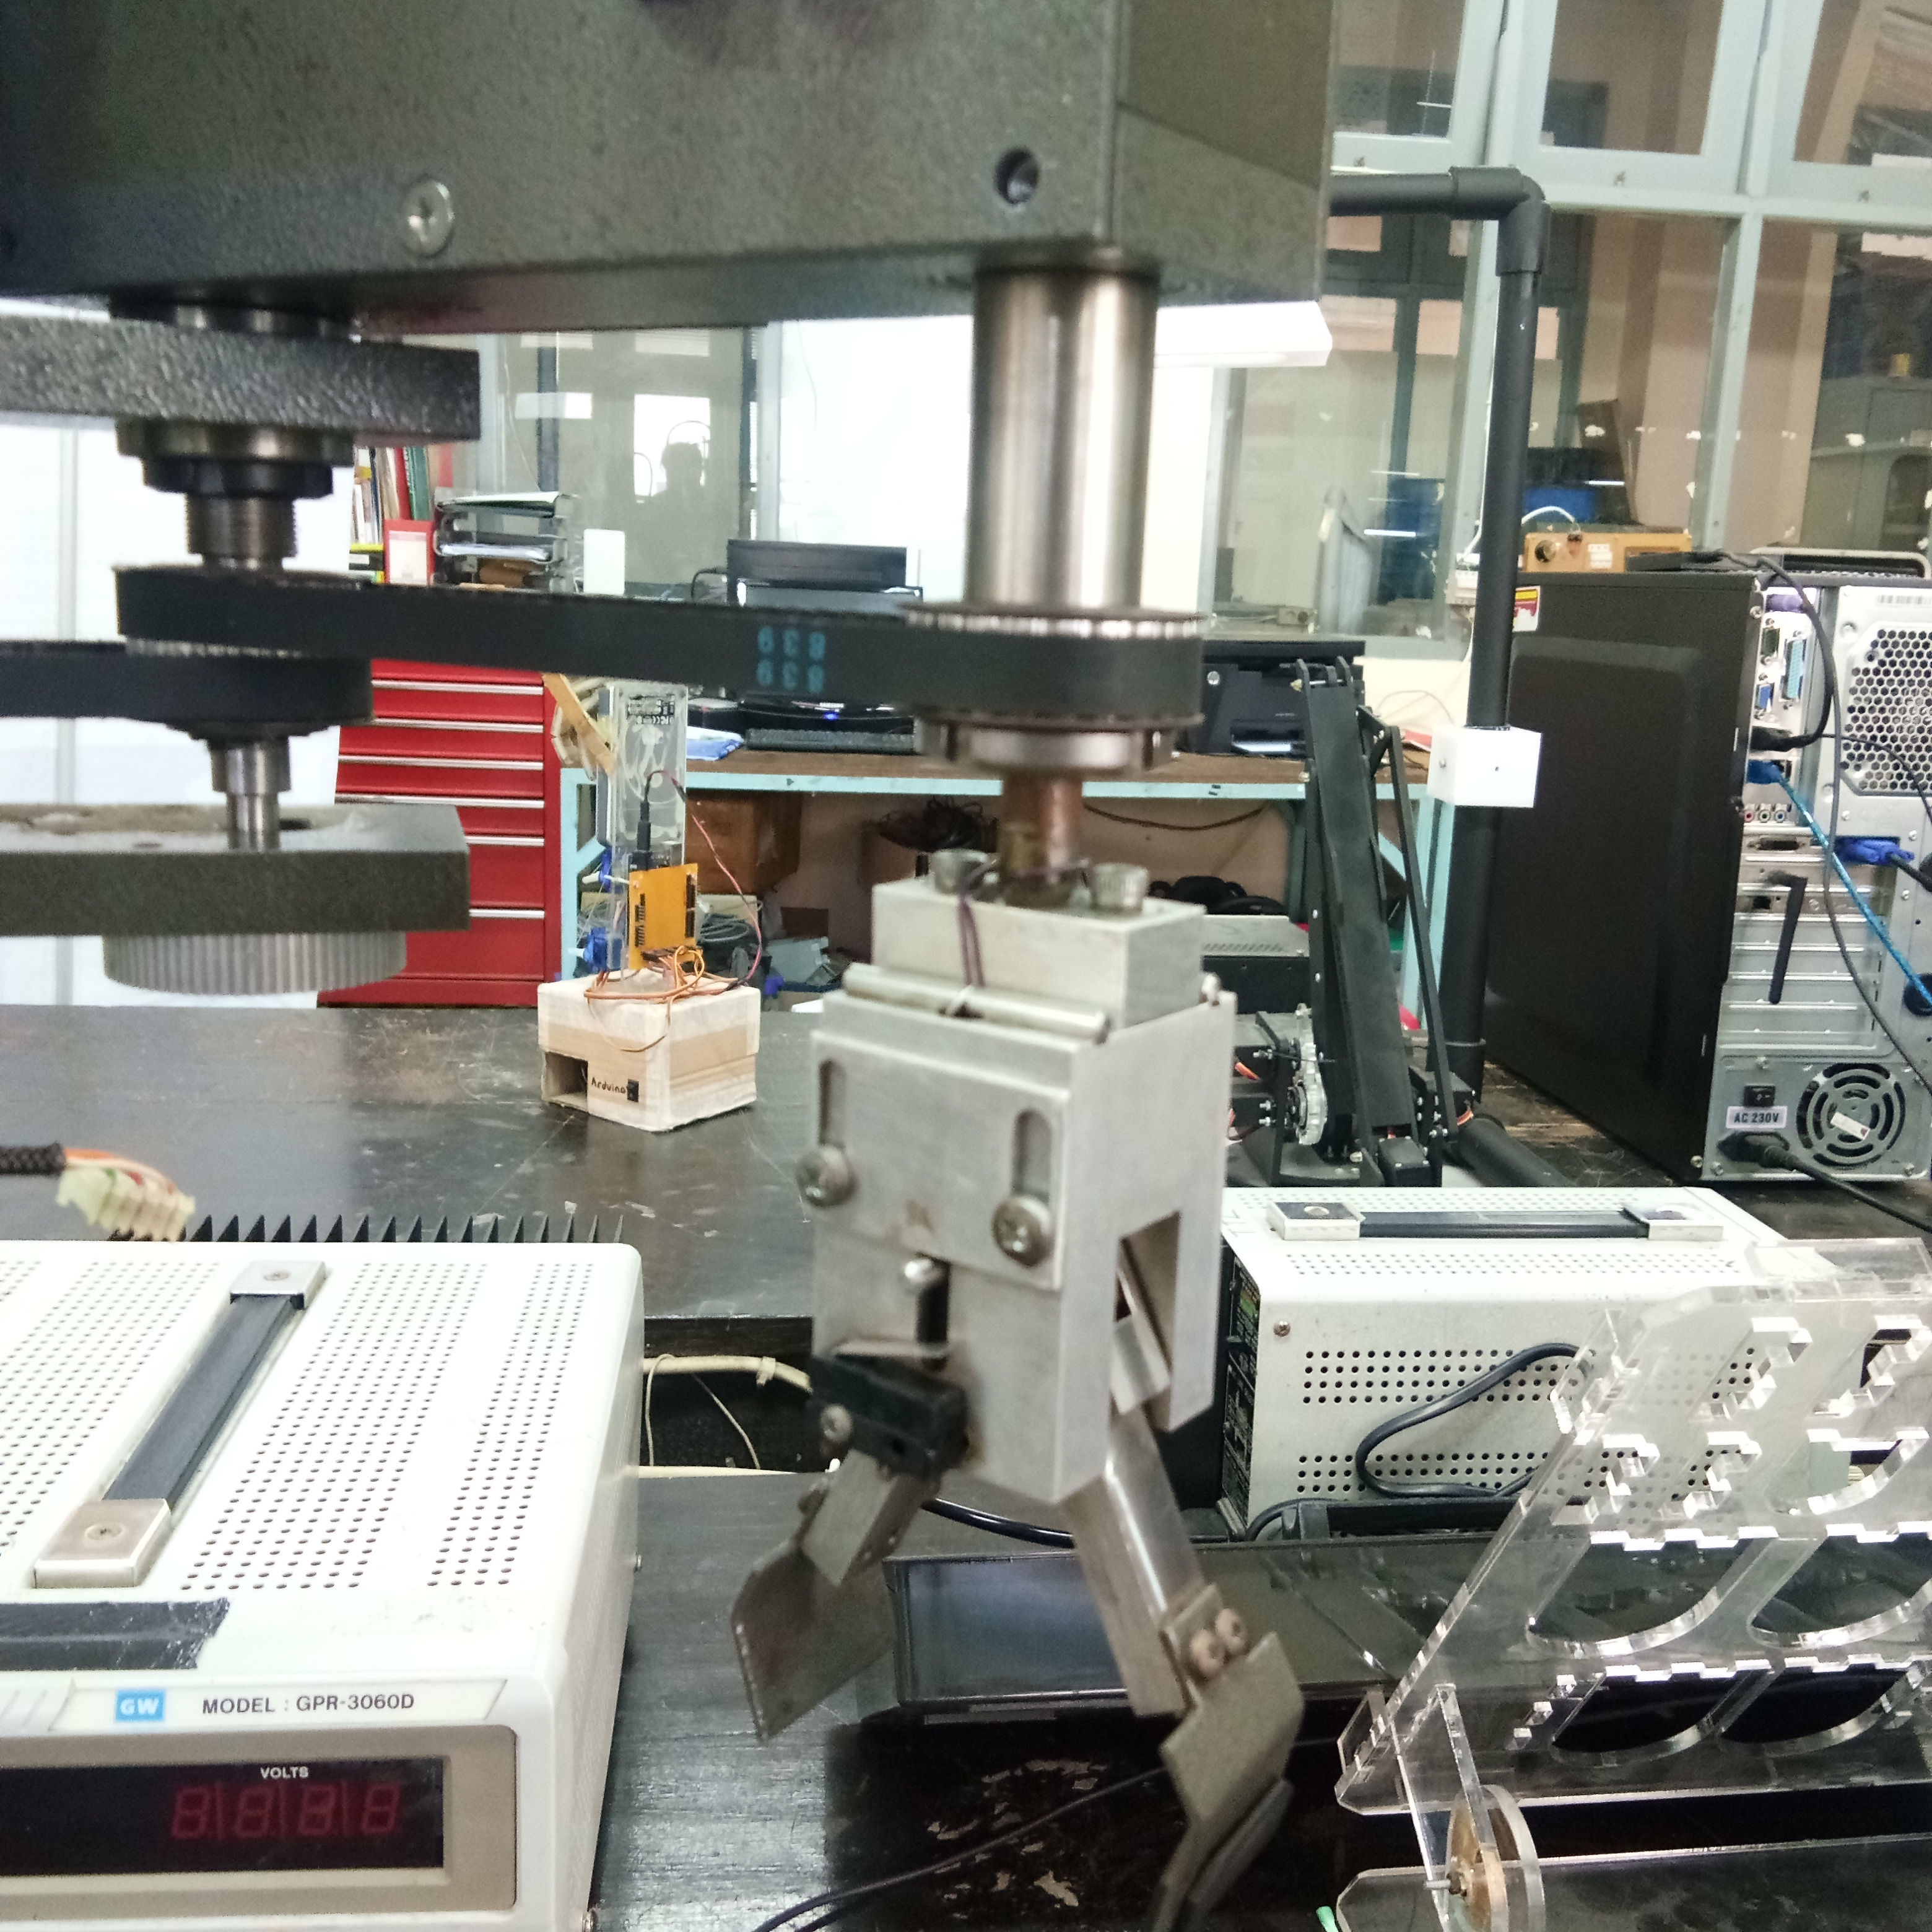
\includegraphics[width=7cm]{gambar/capitsementara.jpg}
	\caption{End-Effector Robot SCARA}
\end{figure}
Semua pergerakan pada \textit{end-effector} ditenagai oleh sebuah tekanan udara yang bersumber dari sebuah kompresor. Tekanan udara diaplikasikan pada sebuah \textit{pneumatic} dengan sistem kerja translasi yang dapat menyebabkan sebuah objek dapat bergerak pada sebuah garis lurus. Gambar 3.7 merupakan bentuk fisik dari pneumatic yang digunakan pada robot SCARA. 
\begin{figure}[H]
	\centering
	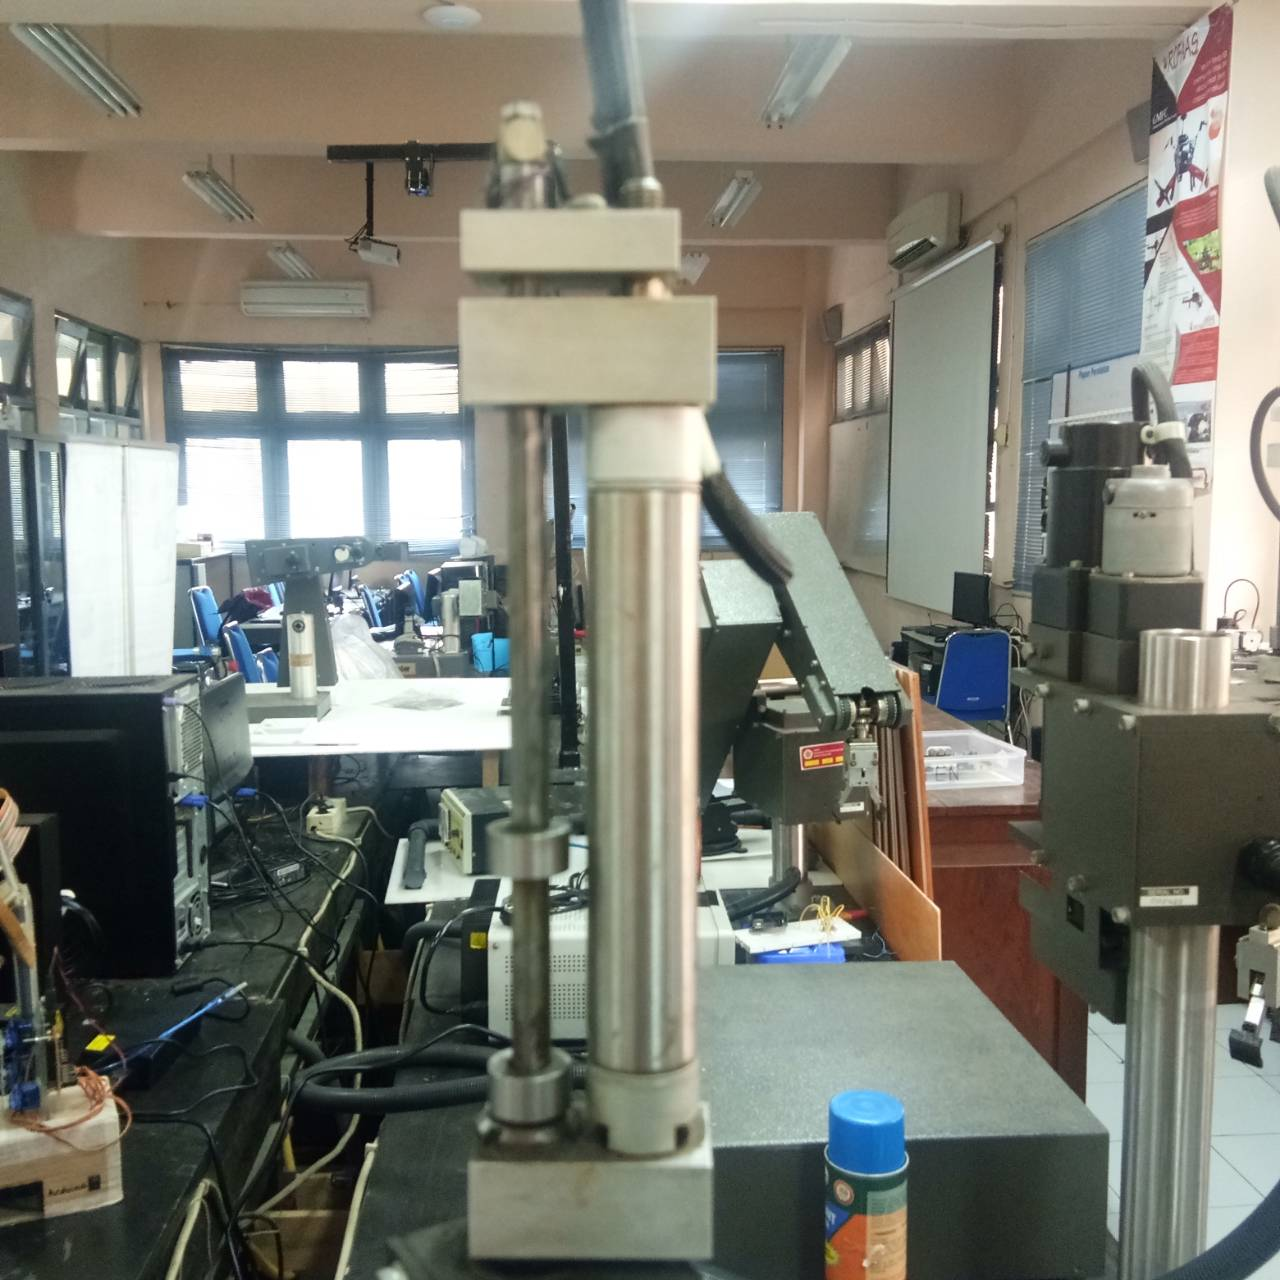
\includegraphics[width=7cm]{gambar/penuamticsementara.jpg}
	\caption{Bentuk Fisik Pneumatic}
\end{figure}
Kompresor yang digunakan untuk menghasilkan sebuah tekanan udara merupakan sebuah kompresor listrik dengan kapasitas 8 bar. Kompresor ini dioperasikan menggunakan sumber tegangan AC. Ketika kapasitas udara sudah terpenuhi, kompresor ini dapat digunakan tanpa menggunakan sumber tegangan tetapi hanya sebatas kapasitas udara yang disimpan. Gambar 3.8 merupakan bentuk kompresor yang digunakan.
\begin{figure}[H]
	\centering
	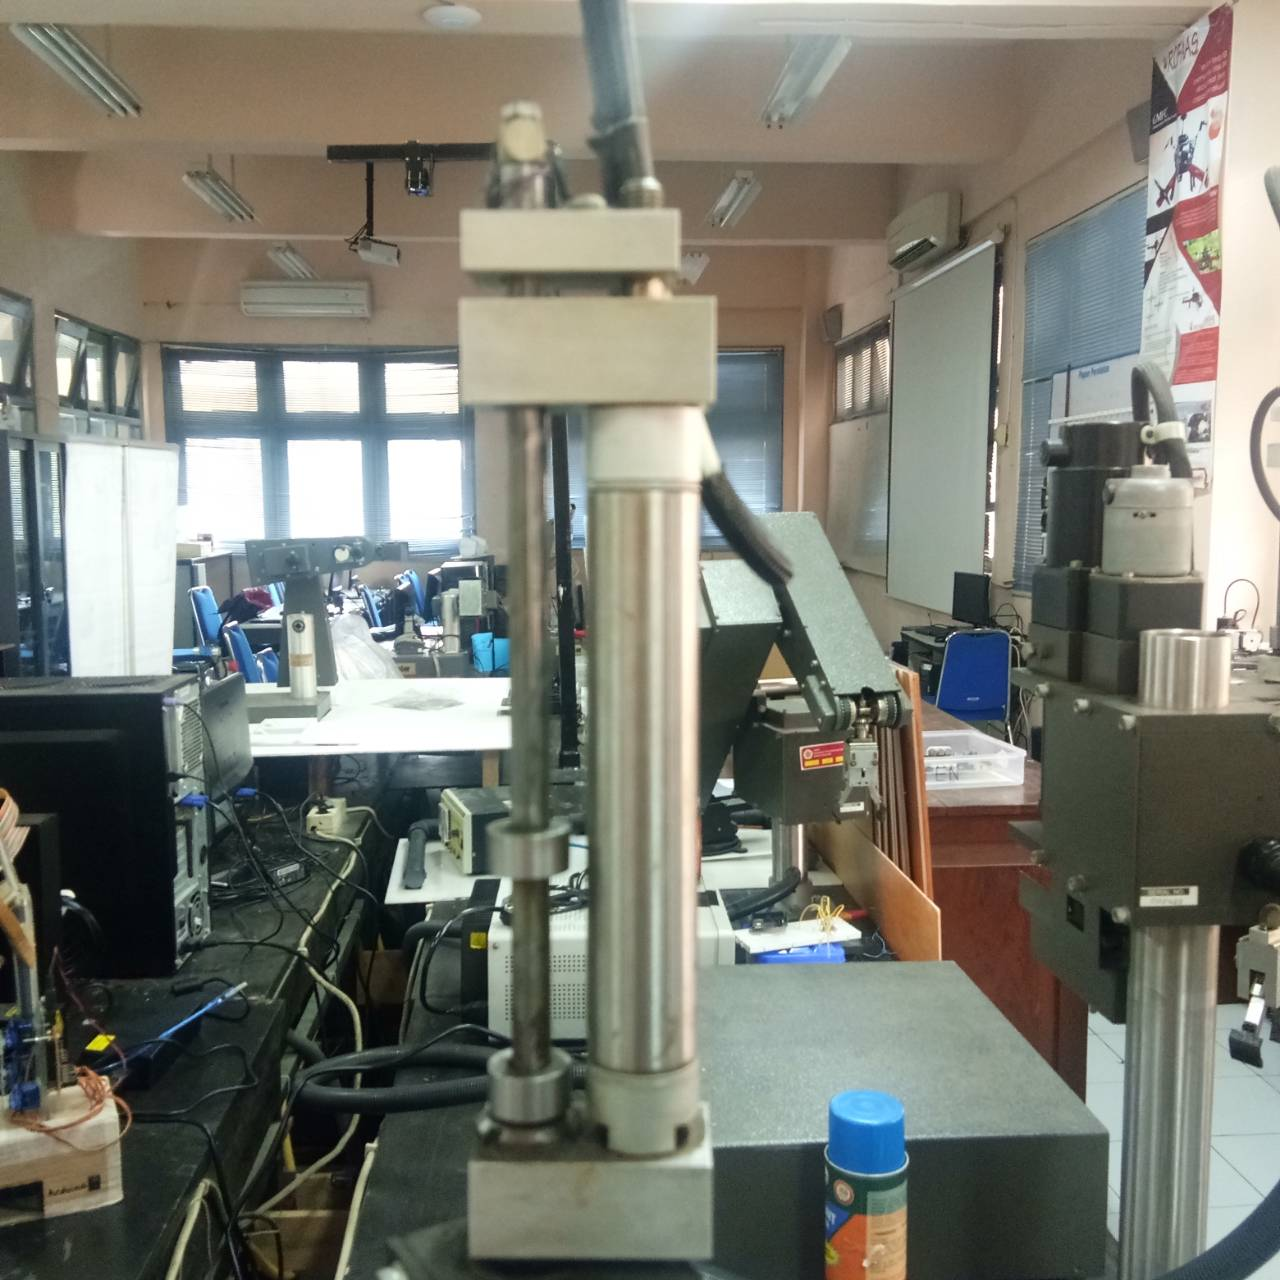
\includegraphics[width=7cm]{gambar/penuamticsementara.jpg}
	\caption{Bentuk Fisik Kompresor}
\end{figure}

Rancangan robot secara keseluruhan ditampilan pada Gambar 3.9 yang merupakan rancangan tampak samping, Gambar 3.10 merupakan rancangan tampak atas dan Gambar 3.11 merupakan rancangan dimensi robot. 
\begin{figure}[H]
	\centering
	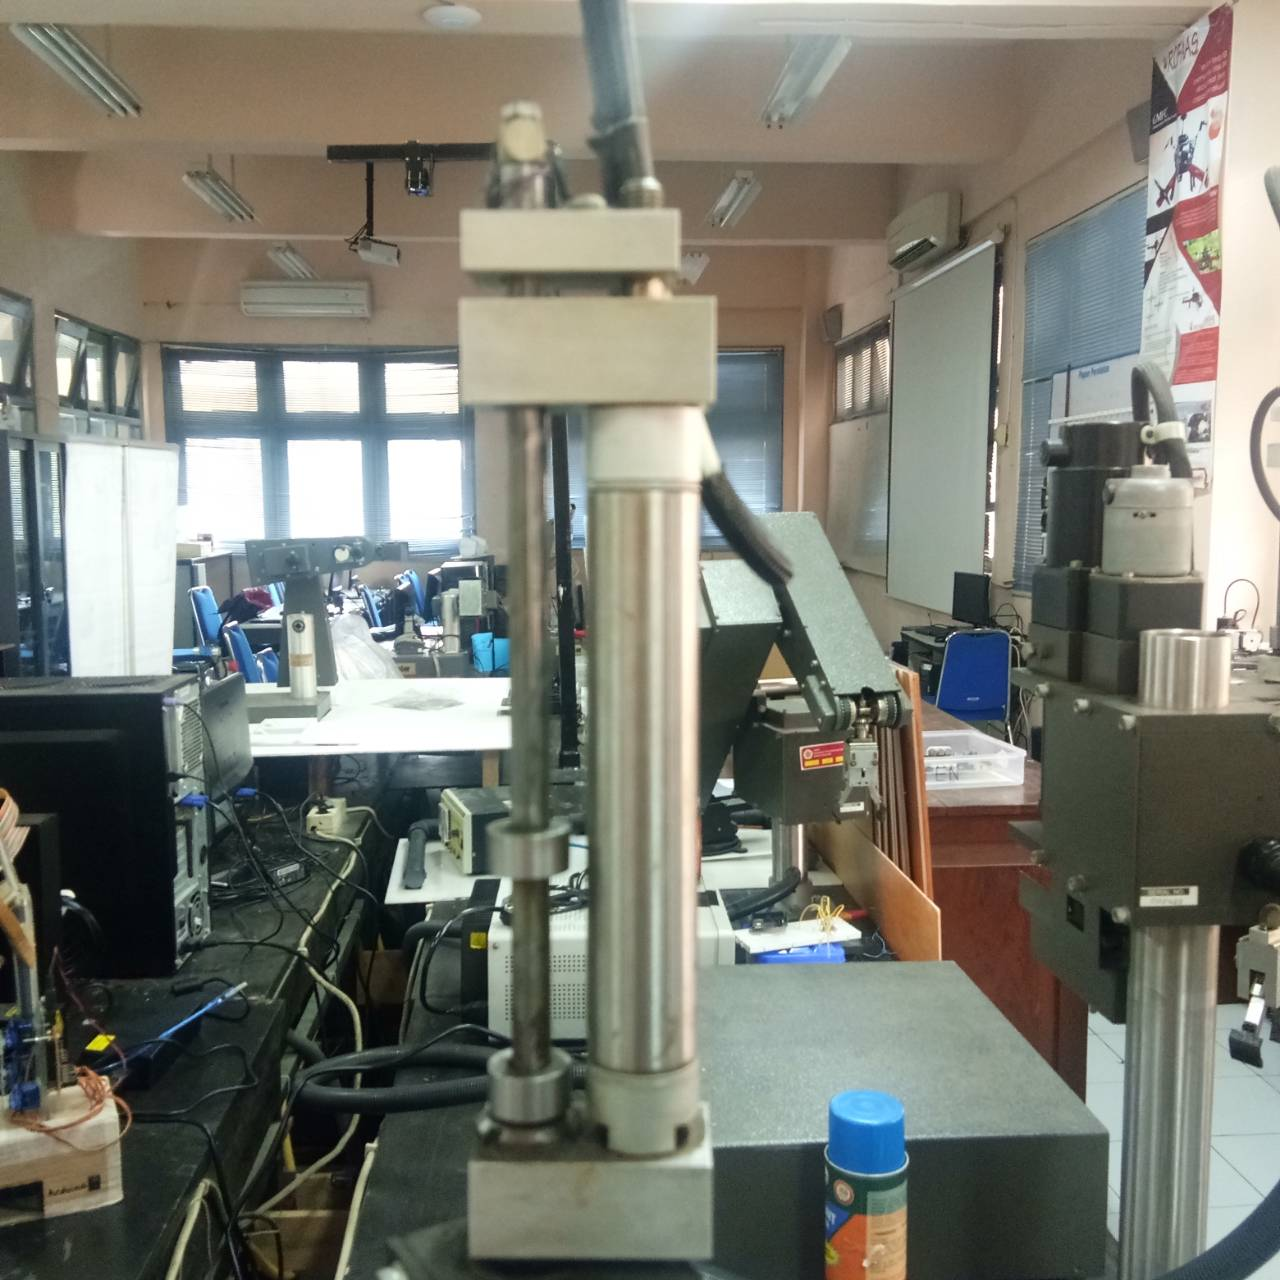
\includegraphics[width=7cm]{gambar/penuamticsementara.jpg}
	\caption{Rancangan Tampak Samping}
\end{figure}

\begin{figure}[H]
	\centering
	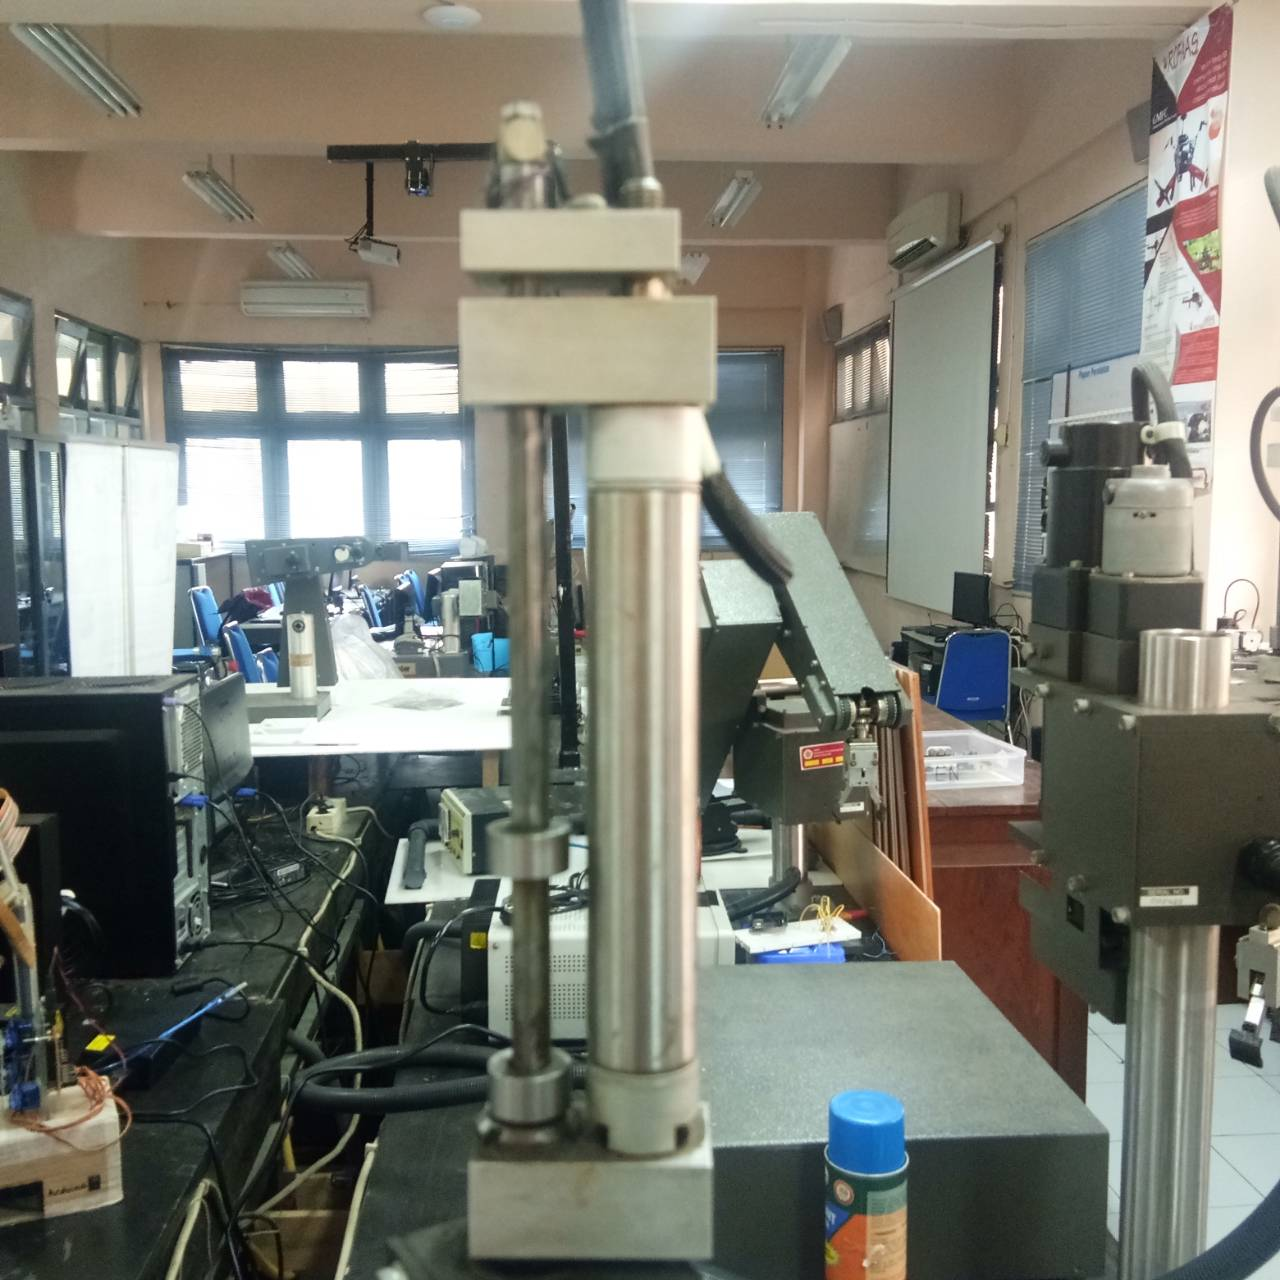
\includegraphics[width=7cm]{gambar/penuamticsementara.jpg}
	\caption{Rancangan Tampak Atas}
\end{figure}

\begin{figure}[H]
	\centering
	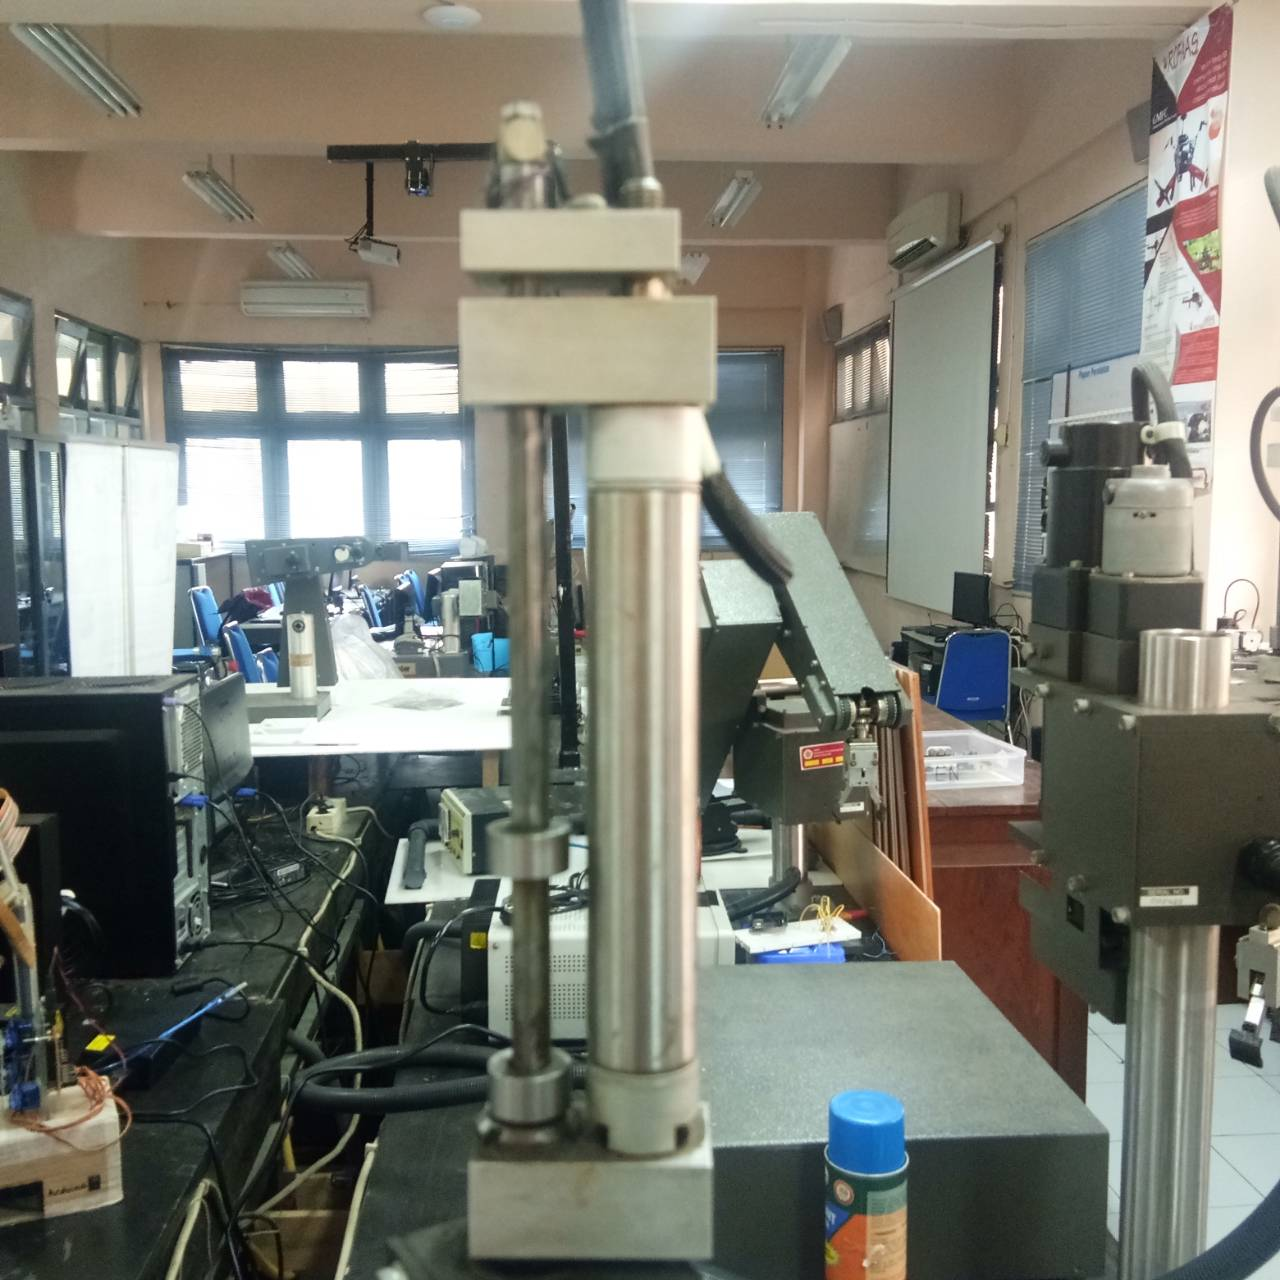
\includegraphics[width=7cm]{gambar/penuamticsementara.jpg}
	\caption{Dimensi Robot}
\end{figure}


